\section{Input analysis}

\subsection{Purpose}
This section provides details for the stochastic inputs for the simulation in accordance with chapter 9 of the textbook \parencite{pensumbok}. The purpose is to identify different elements of the Miller Pain Treatment Center \parencite{MillerPainTreatmentCenter}, organize the available data, fit appropriate probability distributions and justify all assumptions made in the process.

\subsection{Inputs}
The inputs from the Miller Pain Treatment Center can be categorized into three main groups; patient arrivals, treatment times and outcomes for patients (routing decisions). Each of these groups contains multiple stochastic variables that must be modelled probabilistically to capture the random nature of the system.

Patient arrivals are stochastic as they depend on patients arriving early, on time or late for their appointments. This results in queues and system congestion, which must be captured by the model.

Treatment times also vary between patients depending on their conditions and the complexity of the treatment needed. These variables include registration time, vitals, consultation time and treatment, as well as time spent on teaching residents.

Finally, patient outcomes provides stochastic routing decisions in the system. According to their needs, patients follow different paths through the system, resulting in varying resource utilization, waiting times and overall system performance. 

All of these variables must be captured and modelled probailistically to ensure the simulation accurately depicts the system. \autoref{tab:stochastic_vars} summarizes the stochastic variables identified in the Miller Pain Treatment Center, categorized into the three main groups:

\begin{table}[H]
\centering
\small
\begin{tabularx}{\textwidth}{p{4cm} p{2cm} X}
\toprule
\textbf{Variable} & \textbf{Type} & \textbf{Description} \\
\midrule

\multicolumn{3}{l}{\textbf{Service times}} \\
Registration time & Continuous & Time spent on administrative registration \\
Vitals time & Continuous & Time to record patient vitals \\
Physician assistant time & Continuous & Time spent by PA on follow-up patients \\
Check-out time & Continuous & Time to complete visit and paperwork \\
Resident review (new) & Continuous & Time reviewing patient file (new patients) \\
Resident--patient interaction (new) & Continuous & Consultation time with resident \\
Teaching time (new) & Continuous & Teaching interaction between resident and attending \\
Resident--attending interaction (new) & Continuous & Discussion between resident and attending \\
Resident review (return) & Continuous & Time reviewing file (return patients) \\
Resident--patient interaction (return) & Continuous & Consultation time with resident \\
Teaching time (return) & Continuous & Teaching interaction for return patients \\
Resident--attending interaction (return) & Continuous & Discussion between resident and attending \\

\midrule
\multicolumn{3}{l}{\textbf{Routing decisions}} \\
Patient type & Discrete & New, return, or follow-up patients \\
Follow-up requires attending & Discrete & Whether PA consults attending (approximately 50\%) \\
No-show / cancellation & Discrete & Whether patient attends appointment (approximately 10\% no-show) \\

\bottomrule
\end{tabularx}
\caption{Identified stochastic inputs}
\label{tab:stochastic_vars}
\end{table}

\subsection{Extracting relevant data}

The data used in the model is based on the data provided by the Miller Pain Treatment Center \parencite{MillerPainTreatmentCenter}, with the accompanying data from the spreadsheet given. Only data that affects system performance and queue times is used in the model. 

Data for patient arrivals is extracted from the spreadsheet, specifically the deviation between scheduled and actual arrival times. This is essential to capture queue times and congestion in the system, affecting the entire process.

The spreadsheet contains observations for each activity described in the system, with between 90 and 100 observations for each variable. These observations are used to model the service processes in the system.

Finally, relevant routing decisions are also extracted from the case description, to capture the stochastic nature of patient outcomes and their paths through the system. Patient type (new, return or follow-up), decisions regarding follow-up patients and no-show rates are all extracted to determine how patients flow through the system, affecting resource utilization and waiting times.

\subsection{Fitting appropriate statistical distributions}

\begin{figure}[H]
    \centering

    \begin{subfigure}{0.32\textwidth}
        \centering
        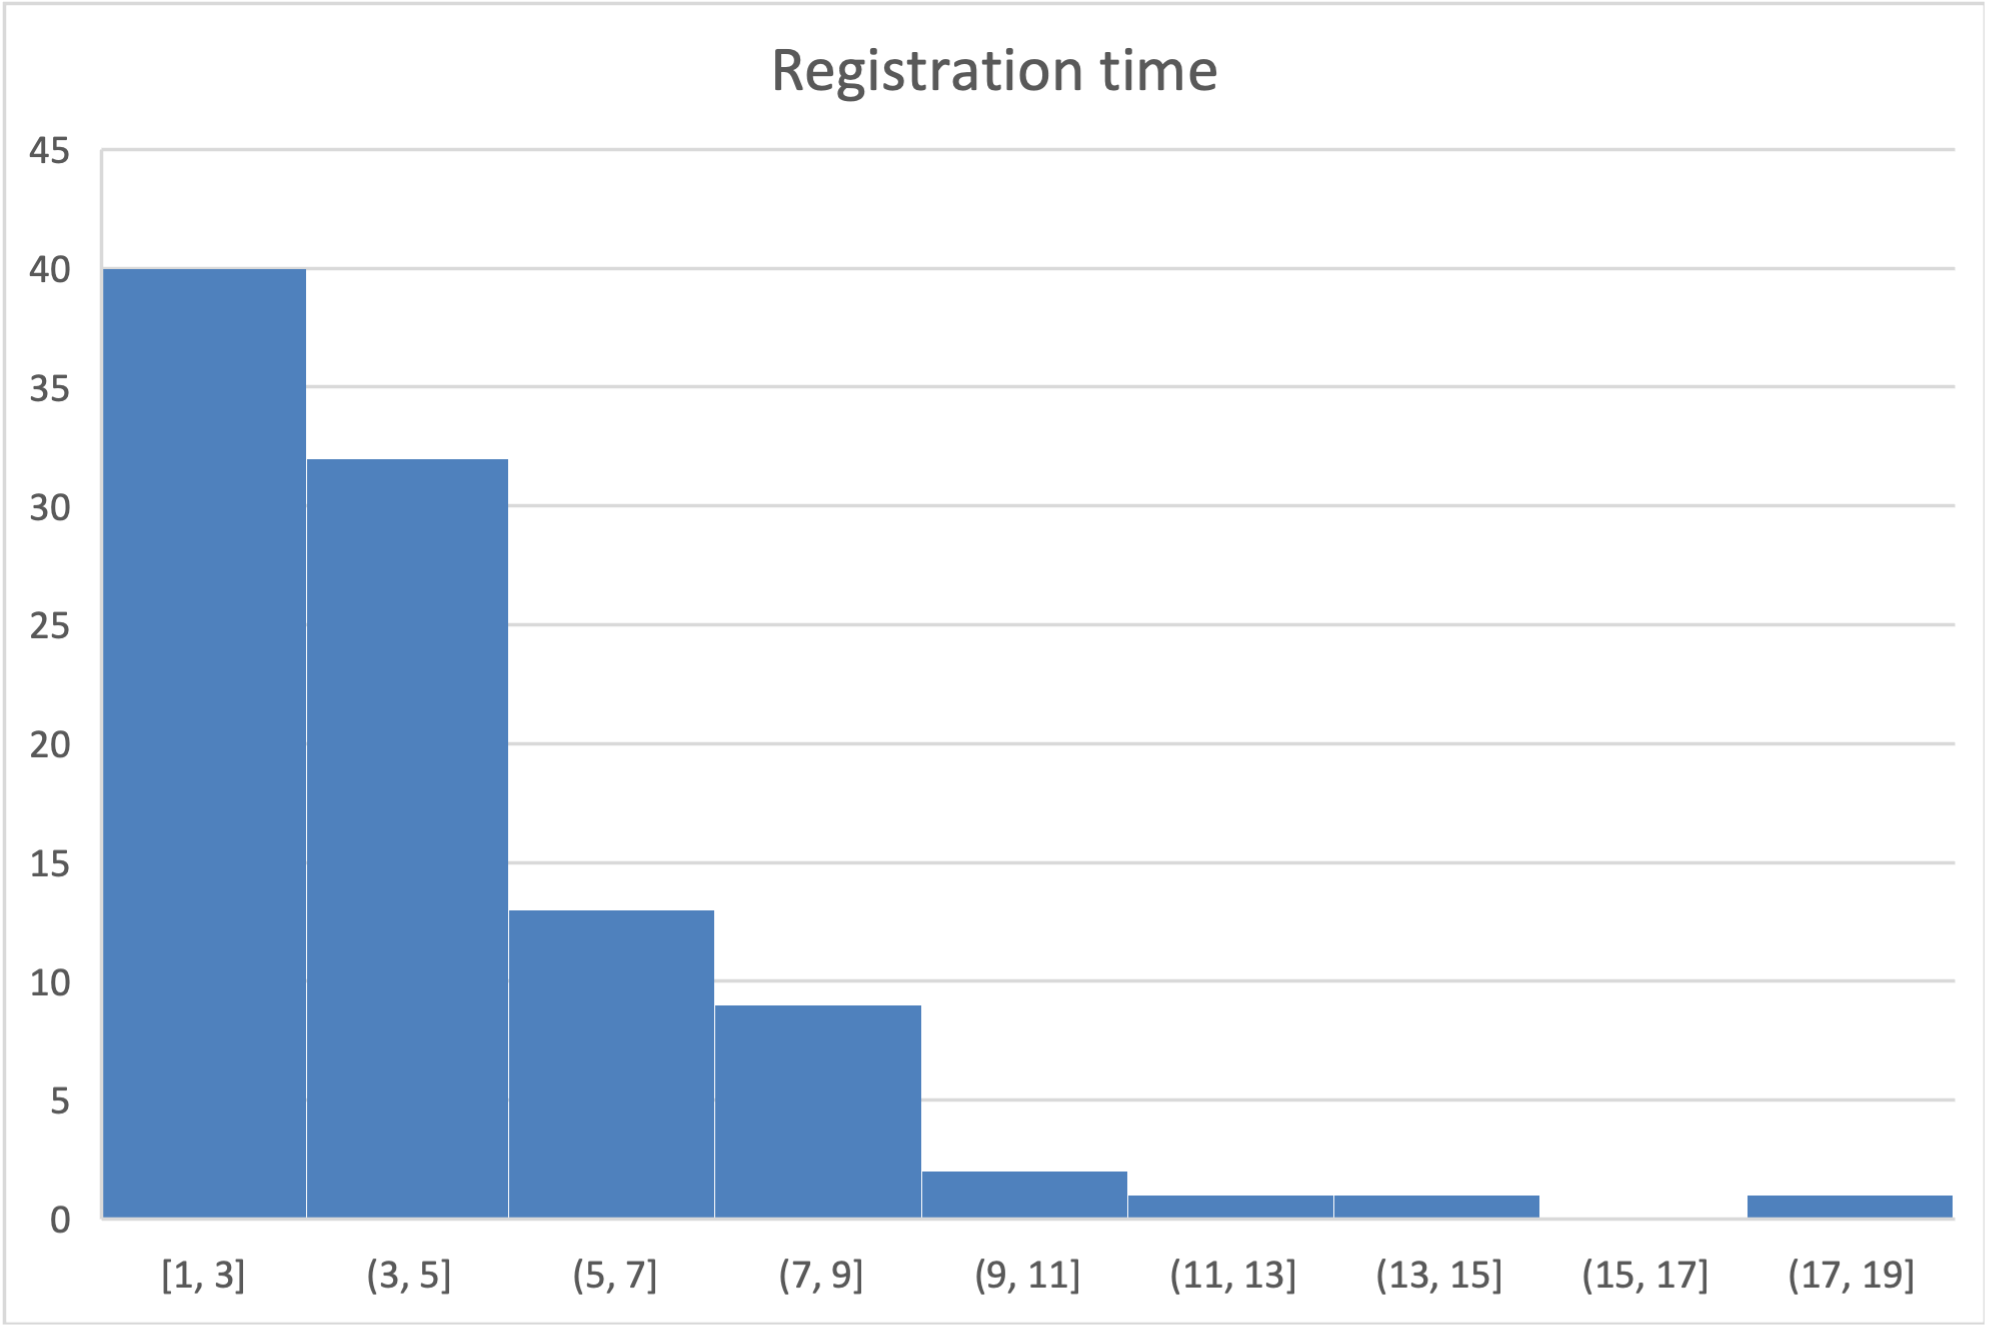
\includegraphics[width=\linewidth]{Inputs/Pictures/RegistrationTime.png}
        \caption{Registration Time}
        \label{fig:reg}
    \end{subfigure}
    \hfill
    \begin{subfigure}{0.32\textwidth}
        \centering
        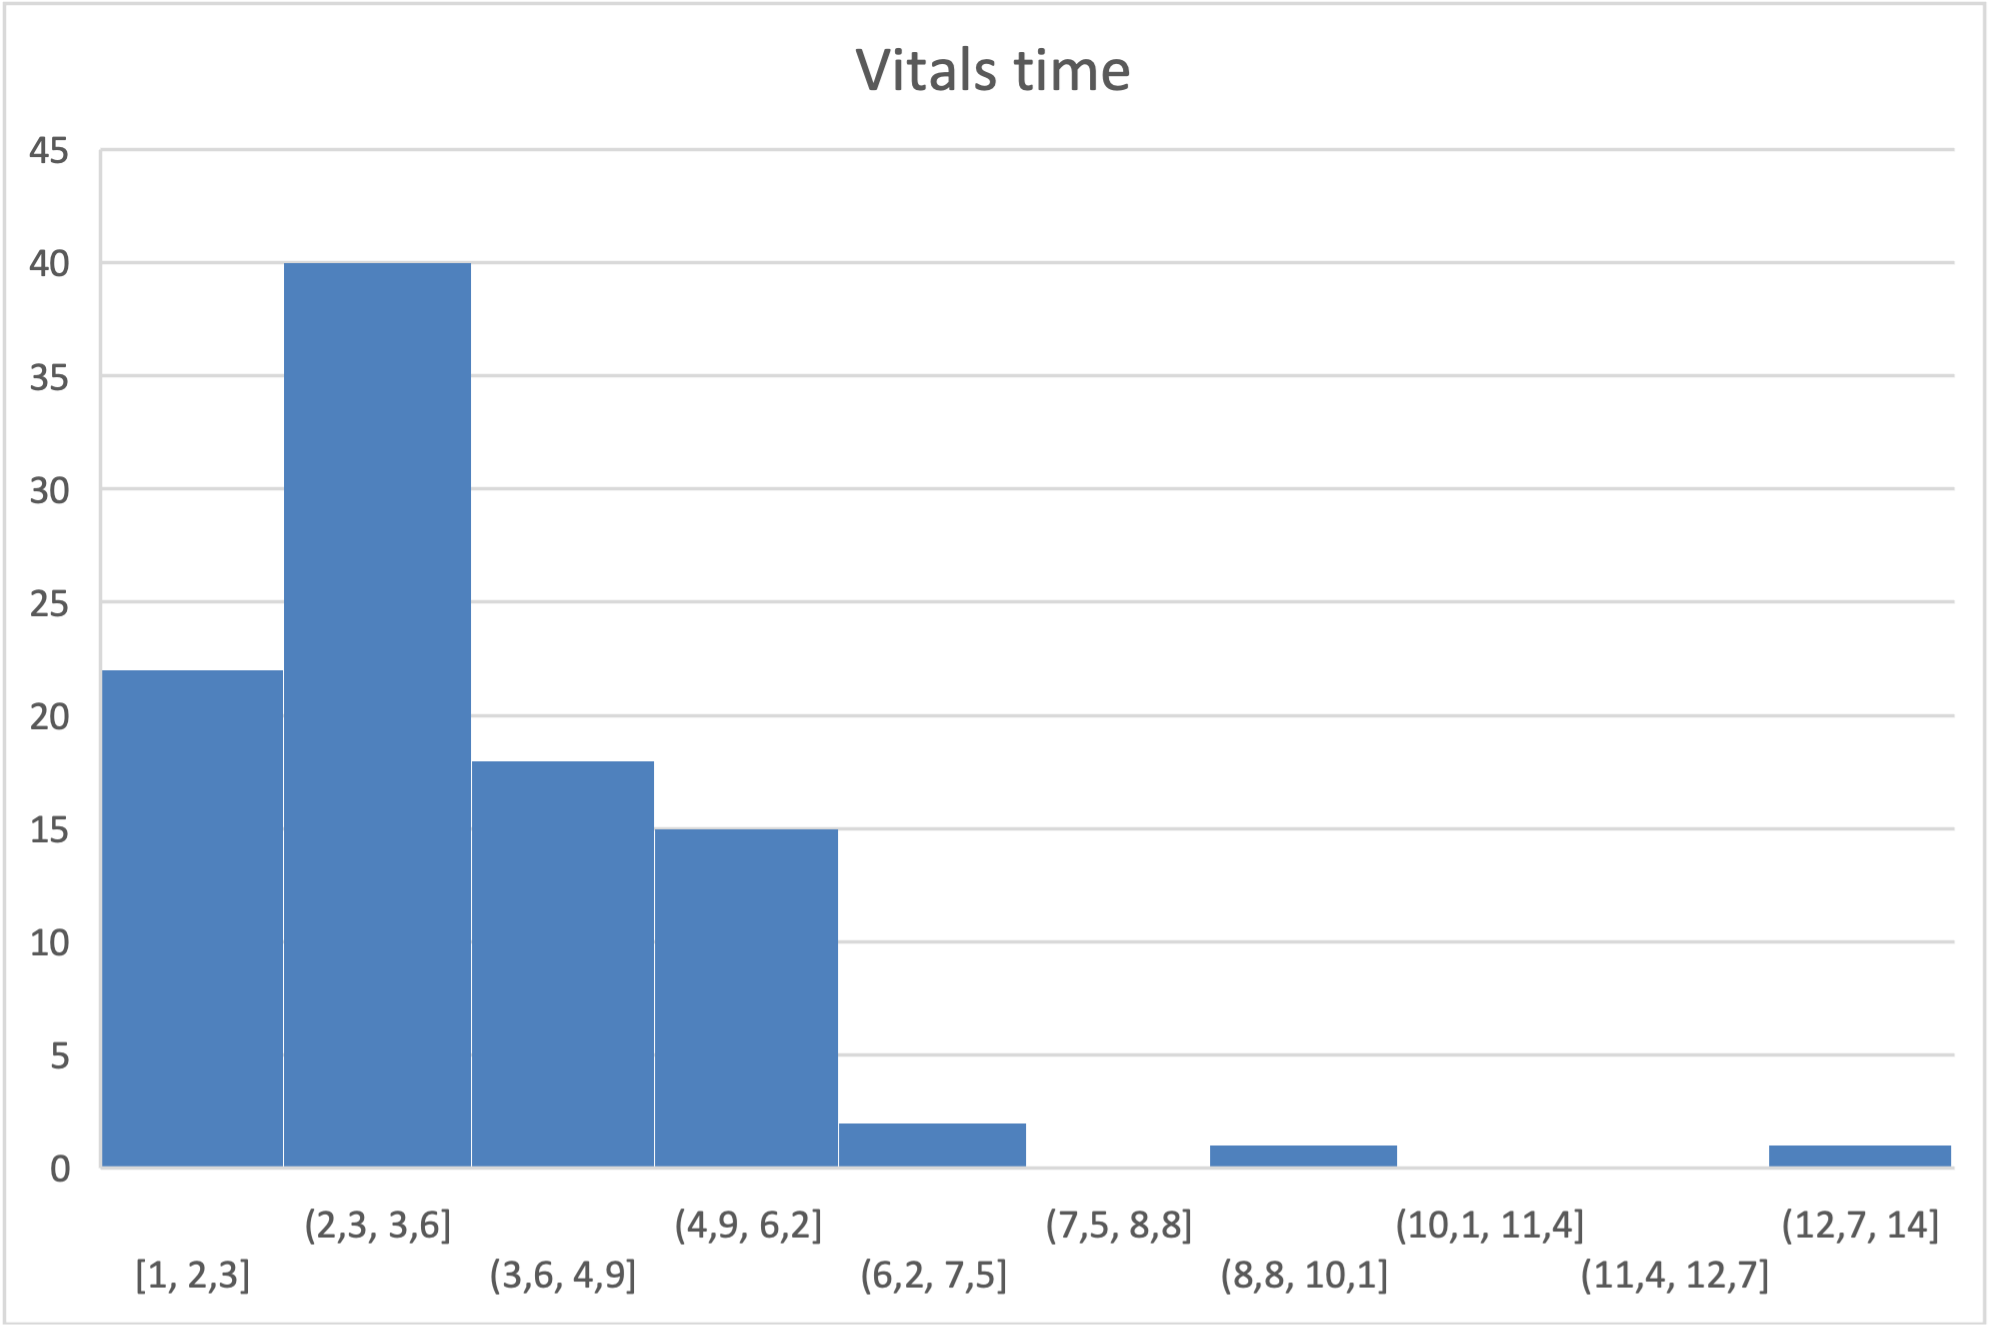
\includegraphics[width=\linewidth]{Inputs/Pictures/VitalsTime.png}
        \caption{Vitals}
        \label{fig:vitals}
    \end{subfigure}
    \hfill
    \begin{subfigure}{0.32\textwidth}
        \centering
        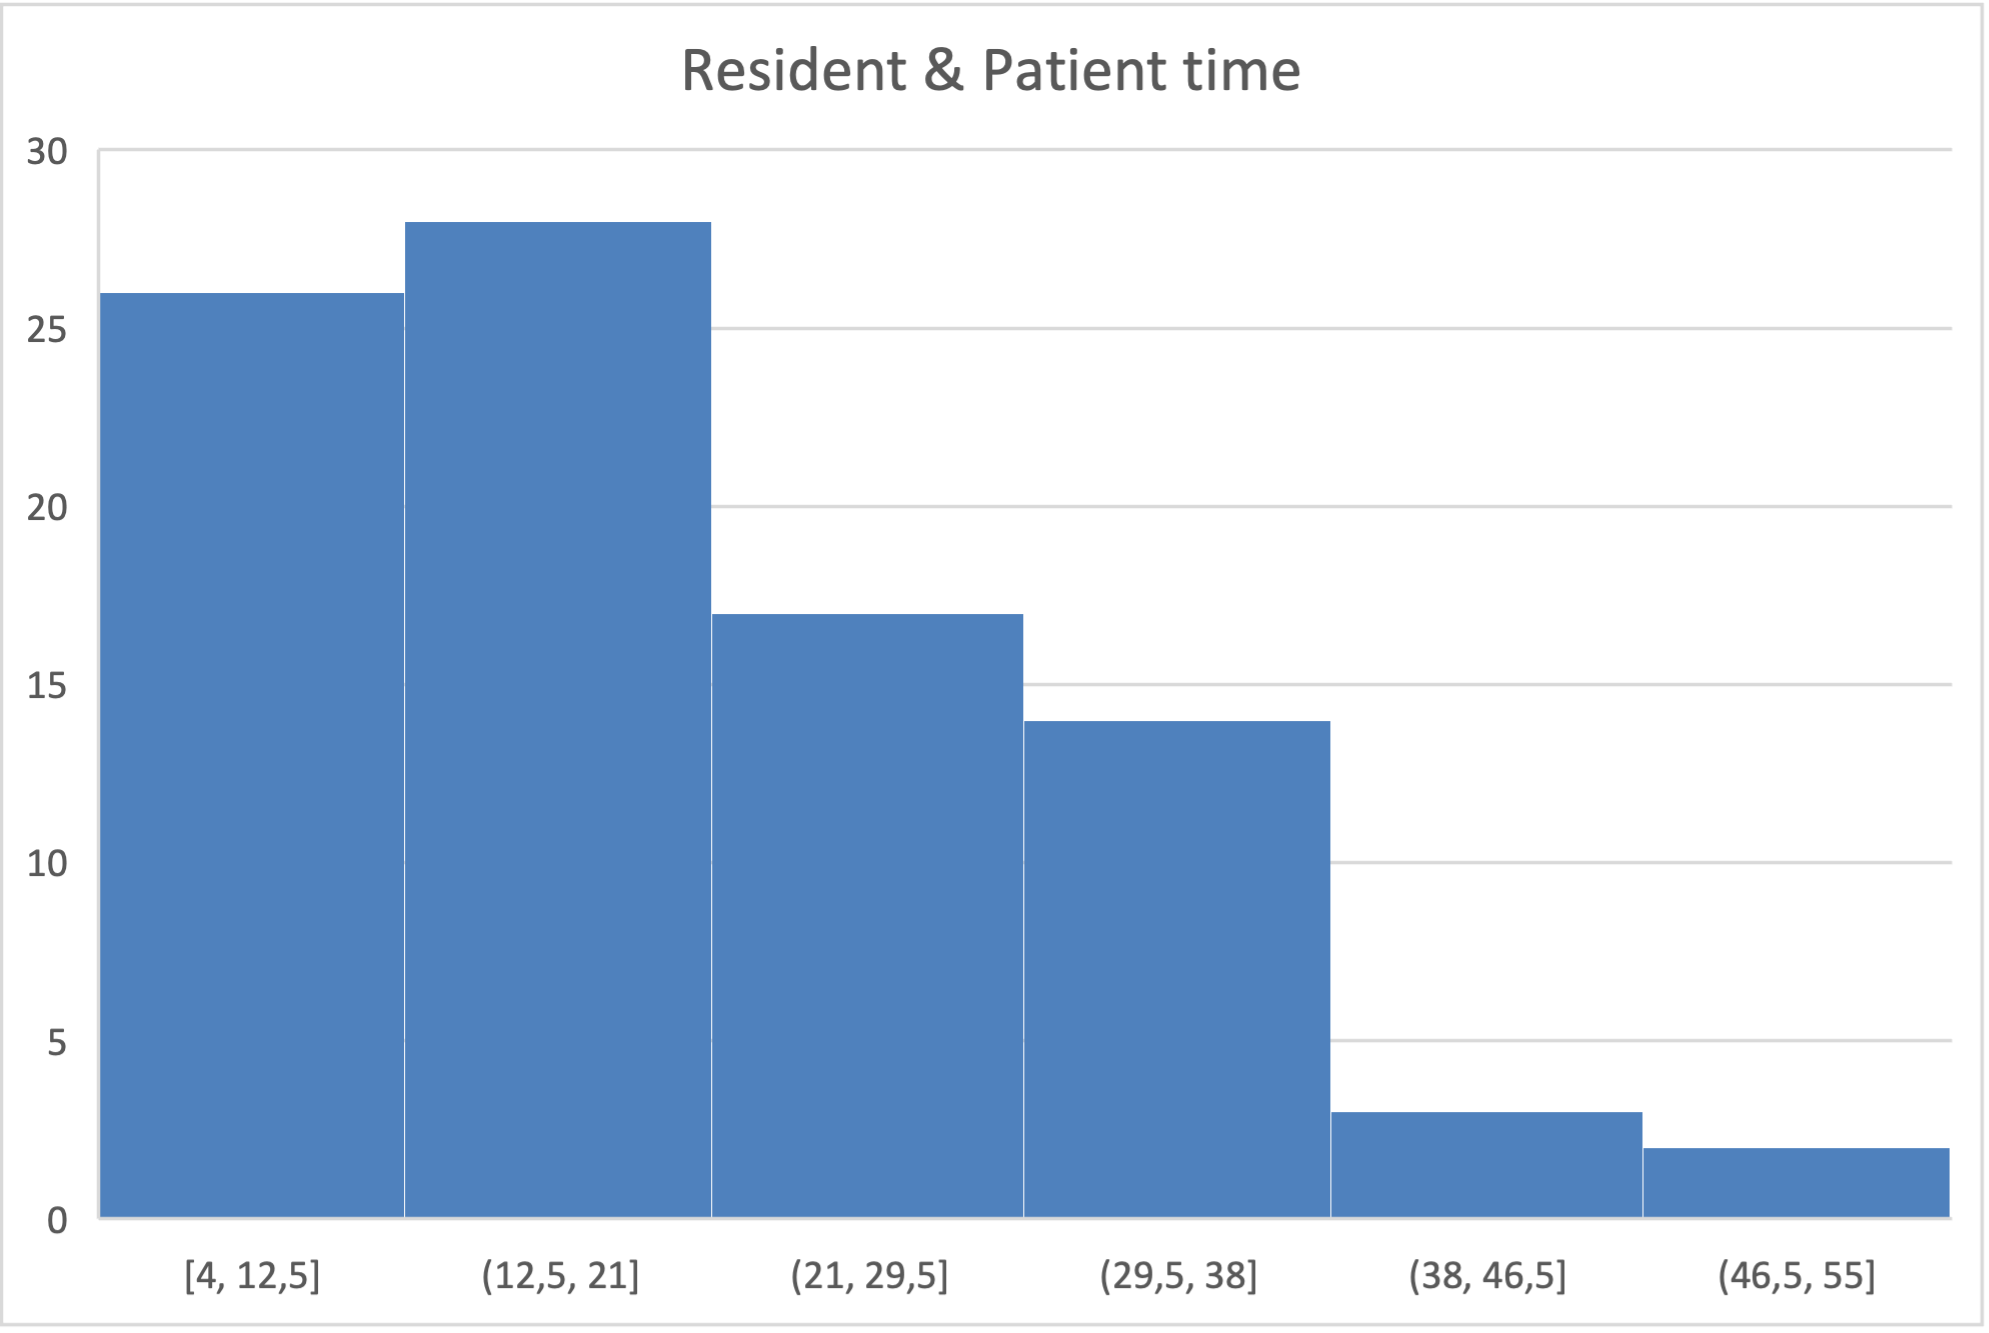
\includegraphics[width=\linewidth]{Inputs/Pictures/ResidentAndPatientTime.png}
        \caption{Resident \& Patient Time}
        \label{fig:resident}
    \end{subfigure}

    \caption{Service times}
    \label{fig:servicetimes}
\end{figure}

To determine a suitable probability distribution, histograms can be used to identify the underlying shape of the data, which can the be compared to known theoretical distributions \parencite[p. 362]{pensumbok}. \autoref{fig:servicetimes} presents histograms for the three example variables registration time (\autoref{fig:reg}), vitals (\autoref{fig:vitals}) and resident \& patient time (\autoref{fig:resident}). 

All three histograms provide a clear right-skewed form with a long tail towards higher values, while most observations are found at lower values. Although the variation differs for the three variables, the overall shape of the data is consitent. This suggests that a positive and flexible distribution, such as Gamma or exponential could be used. We test for these two, in addition to the Lognormal and Weibull distribution.

% To complement the graphical analysis, we calculated descriptive statistics to check this distribution. Our results underline the graphical analysis, highlighting that Gamma would be the best distribution for our model. %Add statistics

\begin{figure}[H]
    \centering
    
\includegraphics[width=0.7\linewidth]{Distributions.png}
    \caption{Fitting distributions}
    \label{fig:distribution}
\end{figure}

\autoref{fig:distribution} shows the histogram of registration times with fitted probability density functions. Using maximium likelihood estimation we can see that Gamma and Lognorm distributions provide the closest fit to the data, as they capture both the right-skewed nature and long tail of the dataset.

\subsection{Goodness-of-fit test}

Using a Kolmogorov-Smirnov goodness-of-fit test we can evaluate the suitability of the Gamma distribution. The KS-test measures the largest absoulte deviation between the empirical and theoritical cumulative probability distribution functions \parencite[p. 423]{pensumbok}. If the deviation is small enough, along with a sufficient p-value, the distribution is considered to be a good suit for the data.

The Gamma distribution is selected as it yeilds a KS statistic of 0.1132 with a p-value of 0.1466, compared to lognormals KS statistic of 0.1195 and p-value of 0.1089. A significance level above 5\% indicates that the null-hypothesis that the data follows a Gamma distribution cannot be rejected, and that the deviation can be explained by randomness \parencite[p. 425]{pensumbok}. This is then done for all variables in the system.

\subsection{Discussing input assumptions}

We make multiple assumptions regarding our dataset to make our model realistic. First, we assume that time is continuous. The dataset provides time in minutes as integers, although it is inherently continuous. This assumption is made to better capture the nature of time, and justifies the use of a continuous distribution such as the Gamma distribution. \\
As some variables, such as teach and resident review contains zero-values, all distributions are fitted with a location parameter of -0.01. Gamma and Lognormal distribution requires strictly positive values, so this is a technical assumption made to ensure all distributions can be fitted.

Second, we assume that the observations are independent of each other, meaning that one patient and their service times does not affect the next patients service time. It is also assumed that service times are steady throughout the observation period, so that the underlying distribution does not change.

Finally, as all distributions are rejected by the KS test for the variable vitals, we use the best distribution available, which is the weibull distribution. This comes at a KS statistic of 0.2028 with a p-value of 0.0005.

\subsection{Final input model}

\autoref{tab:finalinputs} provides all variables with their distributions and parameters. 

\begin{table}[H]
\centering
\begin{tabular}{llcc}
\toprule
\textbf{Variable} & \textbf{Distribution} & \textbf{Shape} & \textbf{Scale} \\
\midrule
Registration & Gamma & 3.069 & 1.415 \\
Vitals & Weibull$^*$ & 2.107 & 3.982 \\
Physicians Assistant & Lognormal & 0.541 & 19.463 \\
Check Out & Gamma & 2.320 & 2.041 \\
Resident Review (New) & Gamma & 1.401 & 7.461 \\
Resident \& Patient (New) & Lognormal & 0.558 & 17.414 \\
Teach (New) & Gamma & 1.879 & 4.184 \\
Resident \& Attending (New) & Gamma & 2.831 & 4.401 \\
Resident Review (Return) & Lognormal & 1.002 & 5.678 \\
Resident \& Patient (Return) & Weibull & 1.740 & 14.665 \\
Teach (Return) & Weibull & 1.173 & 5.438 \\
Resident \& Attending (Return) & Lognormal & 0.738 & 6.974 \\
\bottomrule
\end{tabular}
\\[6pt]
{\footnotesize \textit{$^*$ No distribution with p $>$ 0.05, Weibull chosen as best fit}}
\caption{Final inputs with distributions and parameters}
\label{tab:finalinputs}
\end{table}